% Thesis defence (colloquium), Wed 16 December 2026, 13:00, IKM.
% Filled 2026-10-08 from the thesis as frozen for submission (thesis/).
% Build: pdflatex slides_defense.tex (twice), or .\build_slides.ps1 on IKMHIWI03.
% Speaker script: not written yet (template: speaker_notes_1005.tex).
% CONSTRAINT: total page count <= 20 (main part and appendix). Check the built
% PDF before adding a frame; trim an existing frame rather than tacking one on.
% Rules: CLAUDE.md, "Slides, notes and other documents" (I, not we; no Abaqus
% as thesis work; units on every constant; notation as in the papers; no
% internal labels such as run names or switch numbers).
\documentclass[aspectratio=169,11pt]{beamer}
\usetheme{Madrid}
\usecolortheme{seahorse}
\usepackage{booktabs}
\usepackage{amsmath,amssymb}
\usepackage{bm}
\usepackage{xcolor}
\usepackage{graphicx}
\graphicspath{{assets/}{thesis/figures/}}

\definecolor{c3}{RGB}{30,80,160}
\definecolor{warn}{RGB}{190,40,40}
\setbeamercolor{frametitle}{bg=c3, fg=white}
\setbeamertemplate{navigation symbols}{}
\definecolor{p1}{RGB}{180,83,9}
\definecolor{p2}{RGB}{29,78,137}
\definecolor{p3}{RGB}{62,76,89}
% one message per slide, at the bottom
\newcommand{\takeaway}[1]{\par\vfill\noindent\colorbox{c3!10}{\parbox{\dimexpr\linewidth-2\fboxsep}{\small\textbf{\color{c3}$\rightarrow$}\ #1}}}
% box with a coloured title
\newcommand{\cbox}[3]{\colorbox{#1!8}{\parbox[t][#2][t]{\dimexpr\linewidth-2\fboxsep}{\raggedright #3}}}

\title{Coupling biofilm growth into an existing FEM element}
\subtitle{Master's thesis colloquium}
\author[Keisuke Nishioka]{Keisuke Nishioka}
\institute[IKM, LUH]{%
\small Institute of Continuum Mechanics (IKM), Leibniz Universit\"at Hannover\\[2pt]
\small Examiners: Prof.\ Dr.-Ing.\ Philipp Junker, Dr.-Ing.\ Matthias Wangenheim\\
\small Supervisors: Dr.-Ing.\ Meisam Soleimani, Dr.-Ing.\ Hendrik Geisler}
\date{16 December 2026}

\begin{document}
\maketitle

% --------------------------------------------------------
\begin{frame}{Motivation}
\begin{columns}[T]
\begin{column}{0.55\textwidth}
\begin{itemize}
  \item Peri-implantitis affects about one in five implant patients
        (prevalence 22\,\% and 19.5\,\% in two meta-analyses)
  \item It is driven by multi-species biofilms; a shift towards pathobionts
        such as \textit{P.~gingivalis} goes with disease
  \item A biofilm is also a mechanical body: where it grows unevenly or
        against a stiff substrate, it carries stresses
\end{itemize}
\vspace{6pt}
\textbf{Question:} can the composition of a biofilm, its growth and its
stresses be computed together, in an existing finite element framework?
\end{column}
\begin{column}{0.42\textwidth}
\small
\cbox{p1}{1.6cm}{\textbf{\color{p1}Point model}\\ composition of several species\\ \textcolor{gray}{no space, no stress}}\\[4pt]
\cbox{p2}{1.6cm}{\textbf{\color{p2}Growth field}\\ where the biofilm grows, its stresses\\ \textcolor{gray}{one biofilm variable, no species}}\\[4pt]
\cbox{c3}{1.6cm}{\textbf{\color{c3}This work}\\ both, at every Gauss point of an existing ANSYS element}
\end{column}
\end{columns}
\end{frame}

% --------------------------------------------------------
\begin{frame}{Overview}
\centering
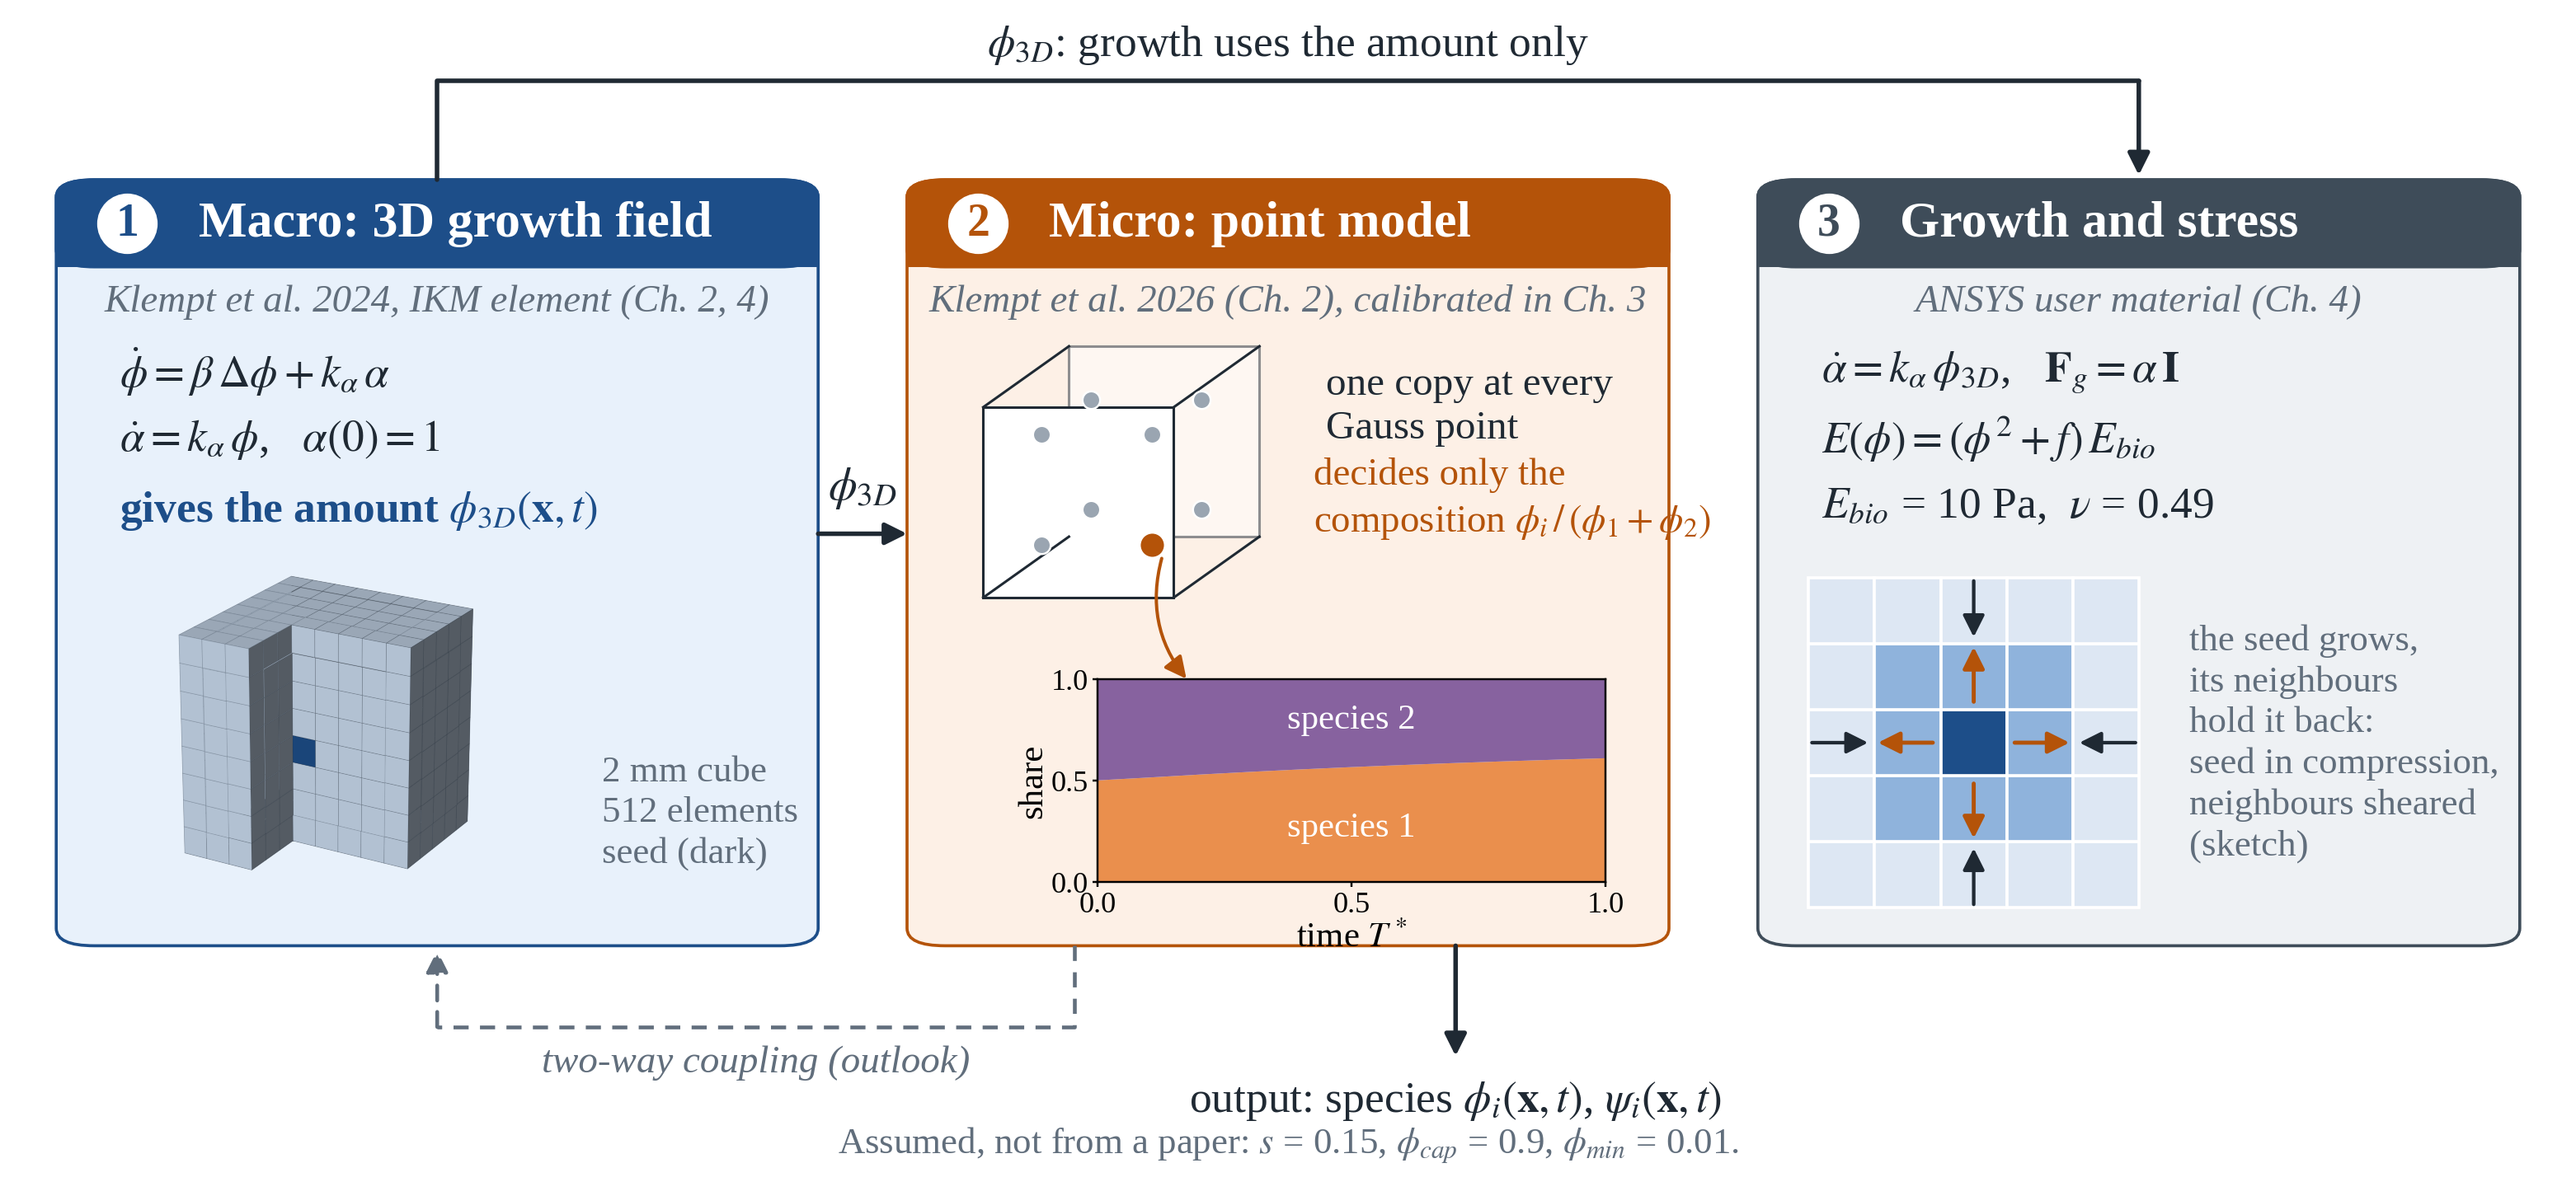
\includegraphics[width=\linewidth,height=0.68\textheight,keepaspectratio]{fig_coupling_schematic_thesis.png}
\takeaway{The field gives the amount $\phi_{3D}$, the point model the composition;
growth and stress use the amount only (one-way).}
\end{frame}

% --------------------------------------------------------
\begin{frame}{Both models from the extended Hamilton principle}
\small
\begin{columns}[T]
\begin{column}{0.5\textwidth}
\textbf{Growth field} (Klempt et al.\ 2024)
\[
\begin{aligned}
&\dot\phi=\beta\nabla^2\phi+k_\alpha\alpha\;(-\text{front term})\\
&\dot c=d\,\nabla^2c-g\,\phi\,c,\qquad \dot\alpha=k_\alpha\phi\\
&\mathbf F=\mathbf F_e\mathbf F_g,\quad \mathbf F_g=\alpha\mathbf I,\quad \alpha(0)=1
\end{aligned}
\]
Stress only from $\mathbf F_e$; growth is $\alpha-1$.
\end{column}
\begin{column}{0.48\textwidth}
\textbf{Point model} (Klempt et al.\ 2026)
\[
\dot\Psi+\Delta+C\;\to\;\operatorname*{stat}_{\dot{\bm\phi},\,\dot{\bm\psi},\,\gamma}
\]
$\Psi=-\tfrac12c^*\bar{\bm\phi}^{\mathrm T}\mathbf A\,\bar{\bm\phi}$,
$\bar\phi_i=\phi_i\psi_i$, $C=\gamma(\sum_l\phi_l-1)$\\[3pt]
the local form of the principle: the principle of the minimum of the
dissipation potential (Junker et al.\ 2014, Hackl 1997)\\[3pt]
$\Rightarrow$ $\mathbf A$ symmetric, $2n+2$ equations per point
\end{column}
\end{columns}
\takeaway{One variational principle for both models: the field for space and stress, its local form for the composition.}
\end{frame}

% --------------------------------------------------------
\begin{frame}{Part 1: calibrating the point model}
\begin{columns}[T]
\begin{column}{0.62\textwidth}
\centering
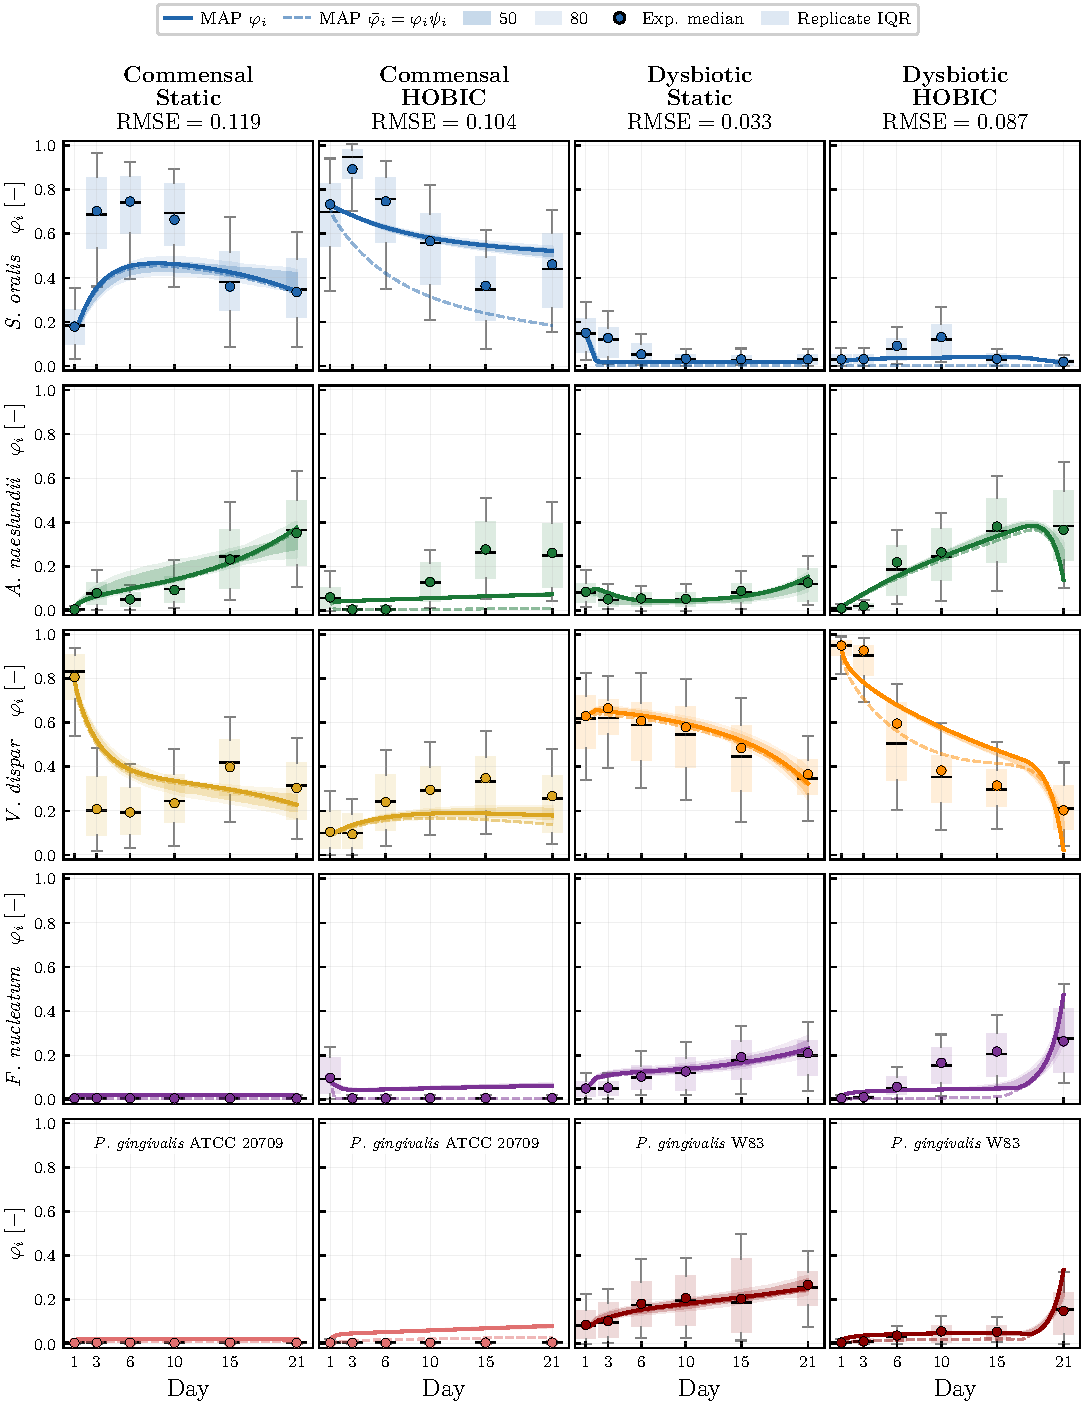
\includegraphics[width=\linewidth,height=0.8\textheight,keepaspectratio]{heine_fits_4cond.pdf}
\end{column}
\begin{column}{0.36\textwidth}
\small
\begin{itemize}
  \item Heine et al.\ (2025): five species, four conditions
        (commensal / dysbiotic, static / flow), days 1--21
  \item 15 coefficients $A_{ij}$ per condition, TMCMC, $10{,}000$ samples
  \item Forward model in JAX on the GPU: about 150 times faster than the CPU
\end{itemize}
\vspace{6pt}
\cbox{c3}{1.5cm}{\small\textbf{\color{c3}Result:} the time courses of all four conditions are reproduced, one symmetric $\mathbf A$ each}
\end{column}
\end{columns}
\end{frame}

% --------------------------------------------------------
\begin{frame}{Part 1: what the calibration gives}
\begin{columns}[T]
\begin{column}{0.55\textwidth}
\centering
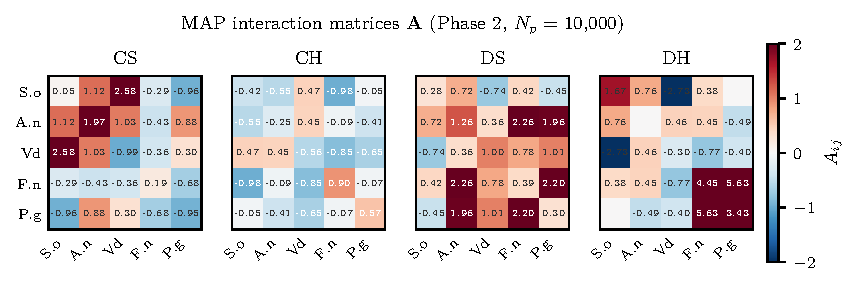
\includegraphics[width=\linewidth,height=0.62\textheight,keepaspectratio]{heine_heatmap_A_4cond.pdf}\\
\small Interaction matrices: the dysbiotic flow condition activates
\textit{F.~nucleatum} $\to$ \textit{P.~gingivalis}
\end{column}
\begin{column}{0.43\textwidth}
\centering
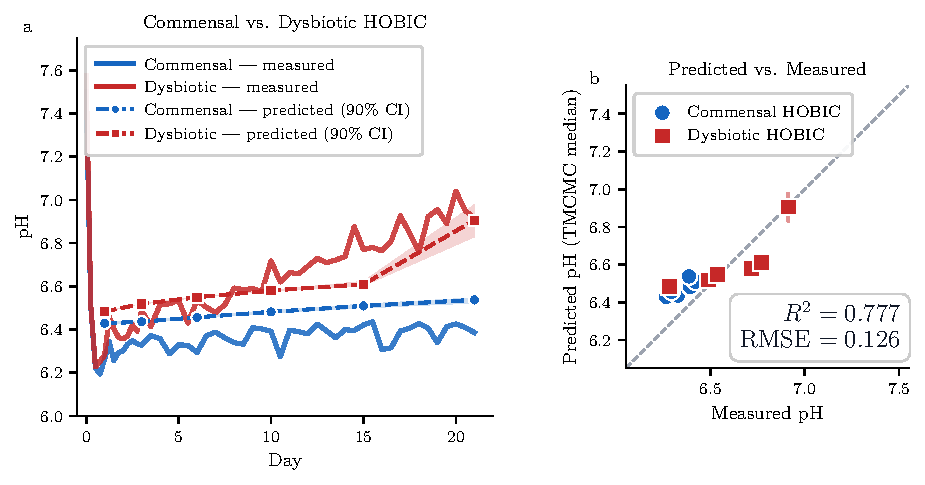
\includegraphics[width=\linewidth,height=0.5\textheight,keepaspectratio]{heine_ph_validation.pdf}\\
\small The pH, not used in the calibration, is predicted with $R^2=0.78$
\end{column}
\end{columns}
\takeaway{\textbf{Prediction} to test: without \textit{F.~nucleatum}, the late growth of
\textit{P.~gingivalis} under dysbiotic flow should be suppressed.}
\end{frame}

% --------------------------------------------------------
\begin{frame}{Part 2: the growth law in ANSYS}
\begin{columns}[T]
\begin{column}{0.38\textwidth}
\small
\begin{itemize}
  \item ANSYS user material: $\mathbf F_g=\alpha\mathbf I$, compressible
        Mooney--Rivlin (neo-Hookean here)
  \item Stiffness of Klempt et al.\ 2024: $E(\phi)=(\phi^2+f)\,E$,
        $E=10$~Pa, $\nu=0.49$, $f=10^{-3}$ (floor, added in this work)
  \item One element against closed forms: constrained growth gives
        $\sigma=-1.0193\times10^{-4}$~MPa as predicted
\end{itemize}
\end{column}
\begin{column}{0.6\textwidth}
\centering
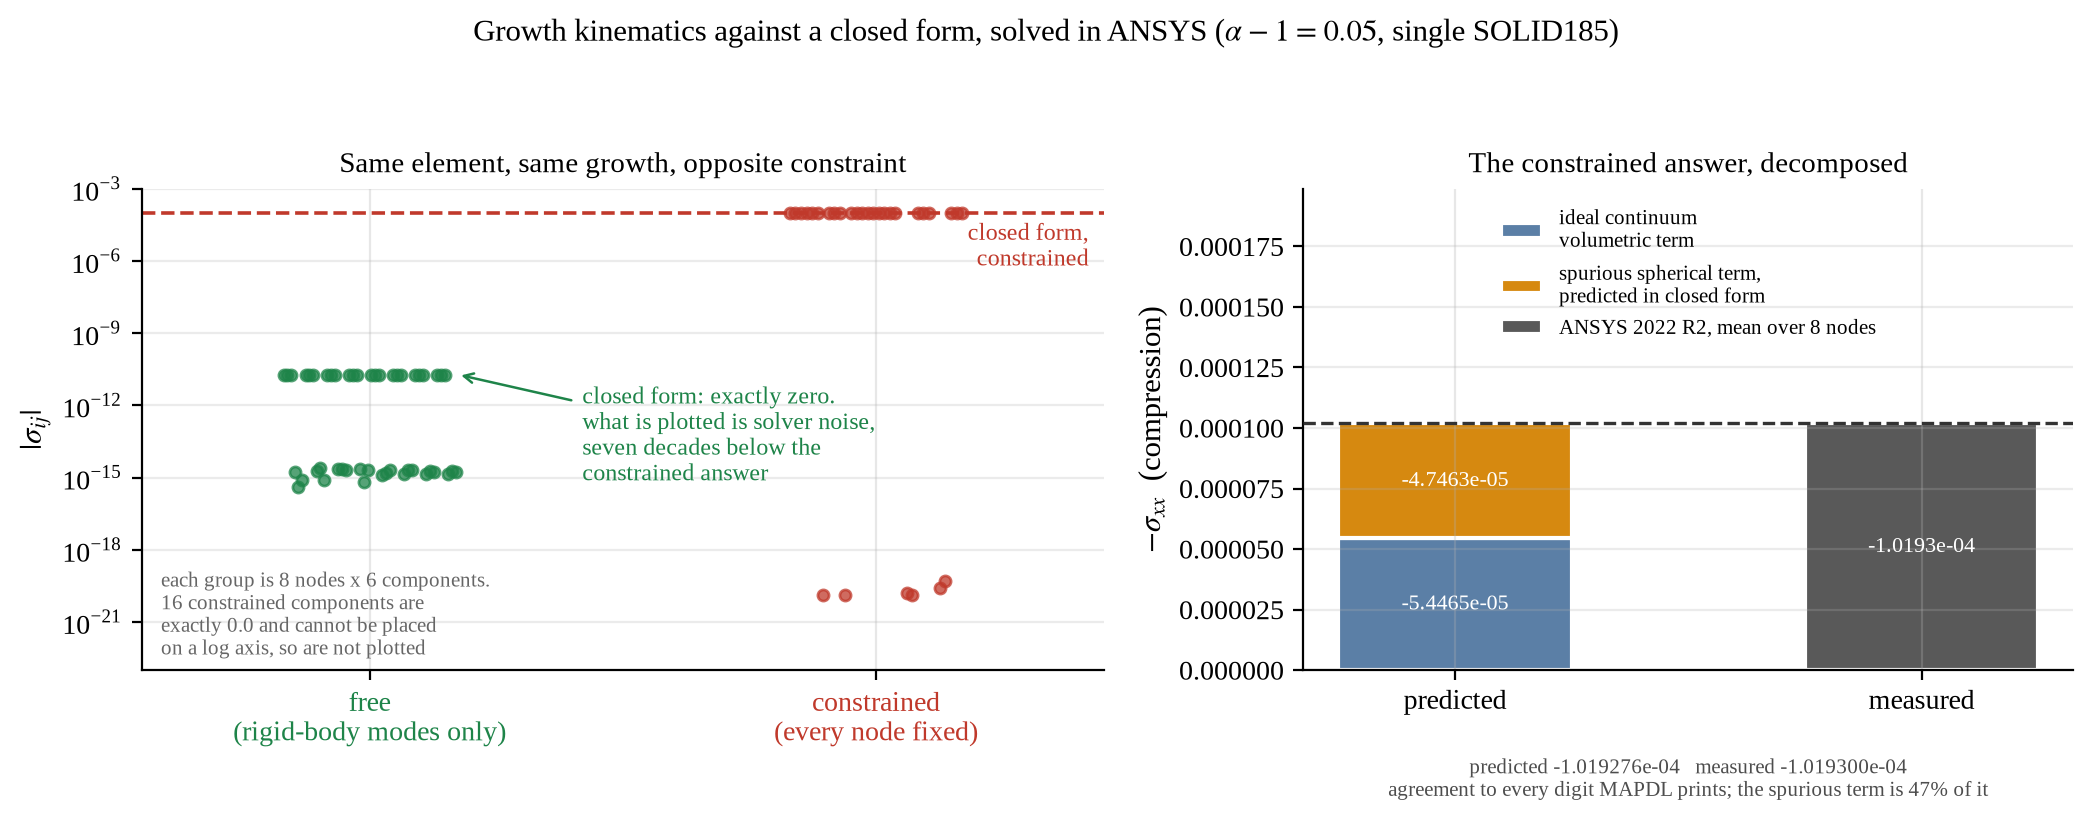
\includegraphics[width=\linewidth,height=0.72\textheight,keepaspectratio]{v222_closed_form.png}
\end{column}
\end{columns}
\takeaway{The growth law in ANSYS matches the closed forms: free growth stays stress free, constrained growth gives the predicted pressure.}
\end{frame}

% --------------------------------------------------------
\begin{frame}{Part 2: coupling into the IKM element}
\begin{columns}[T]
\begin{column}{0.56\textwidth}
\centering
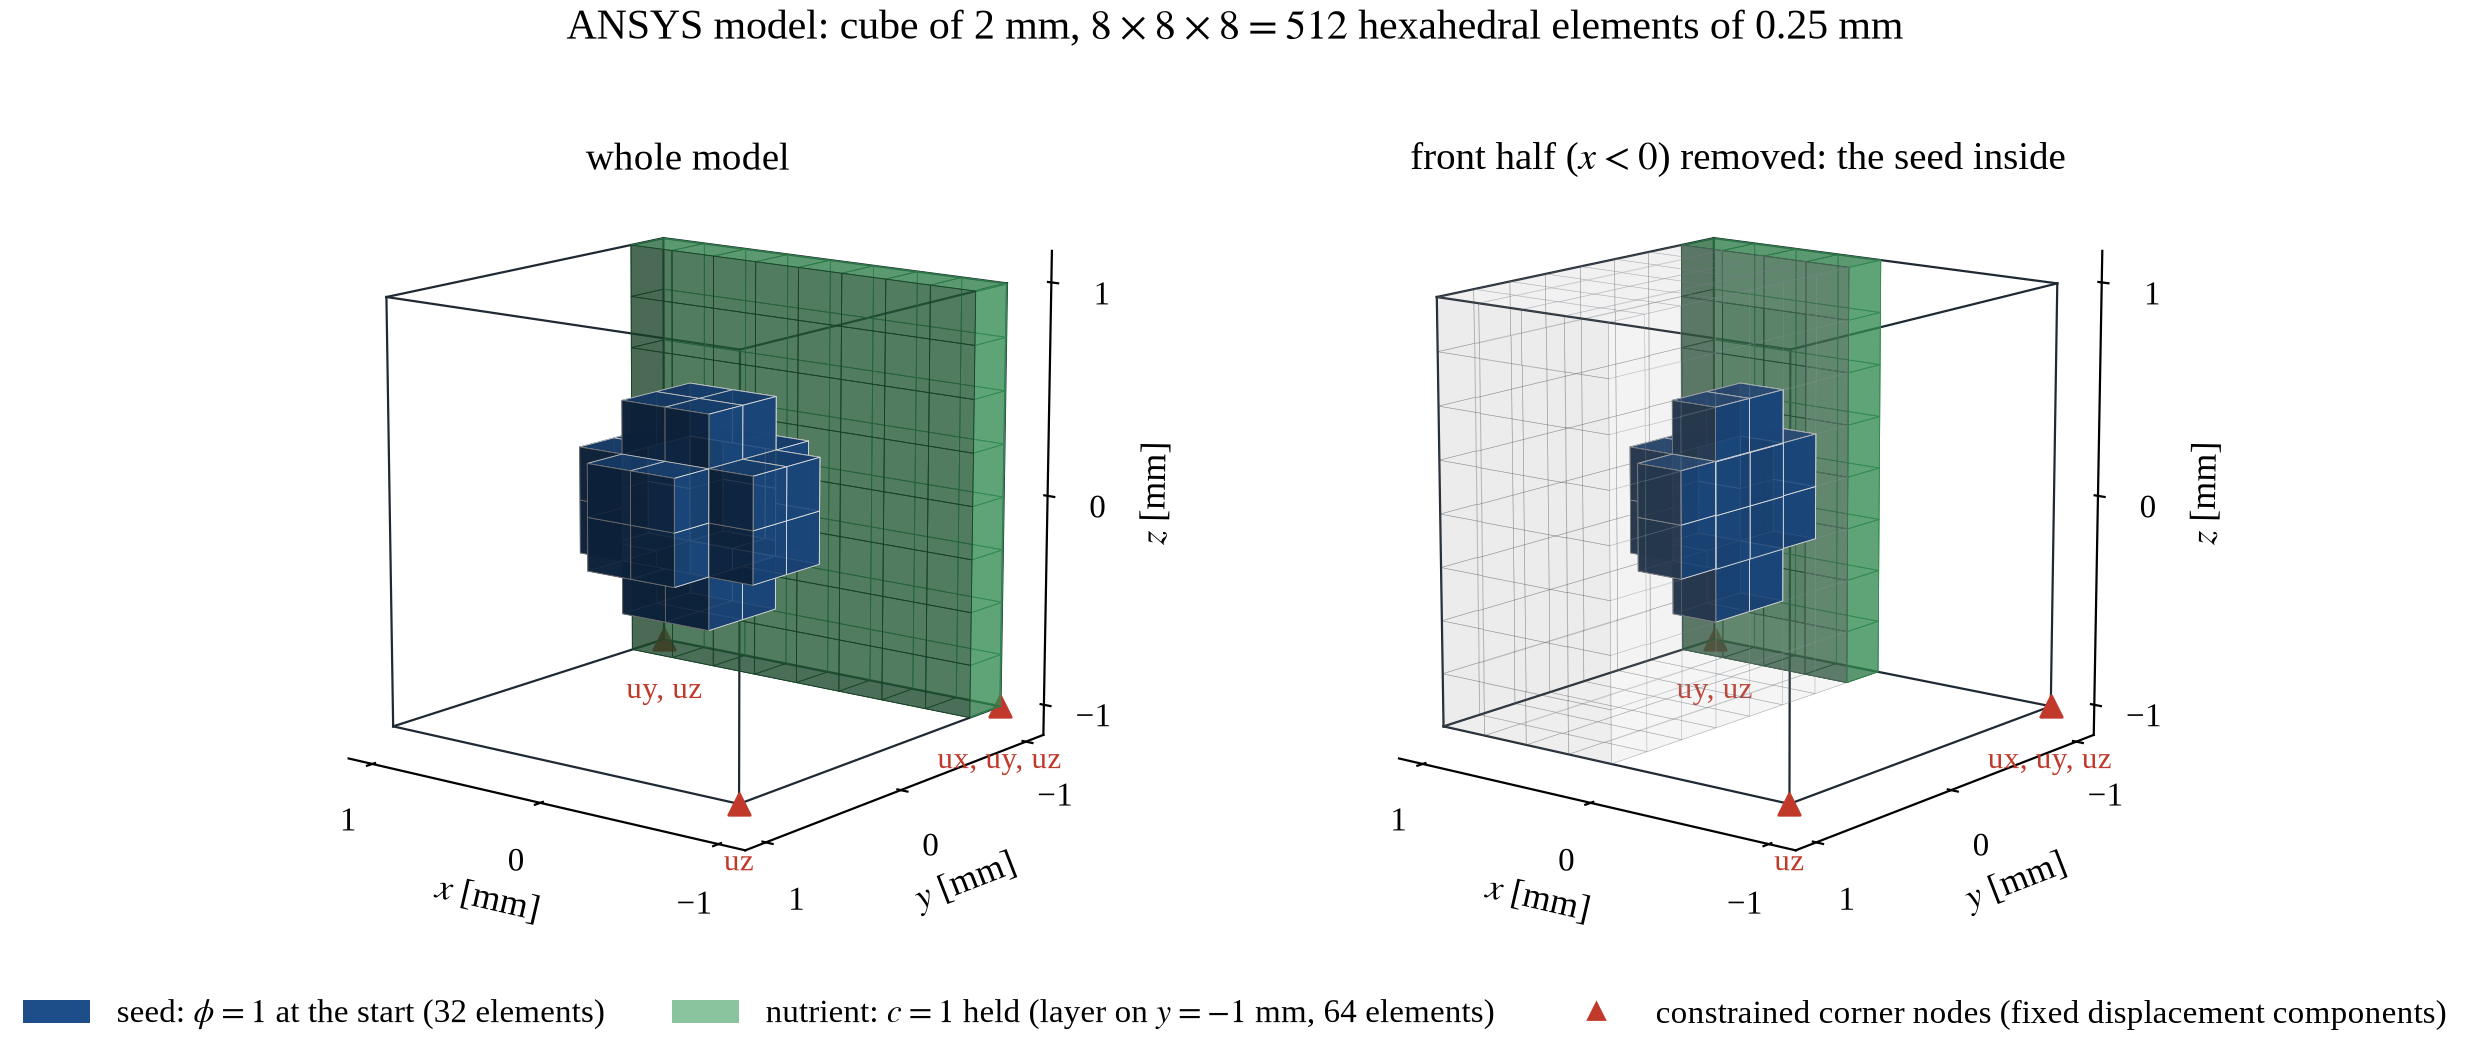
\includegraphics[width=\linewidth,height=0.72\textheight,keepaspectratio]{fig_model_setup.png}
\end{column}
\begin{column}{0.42\textwidth}
\small
\begin{itemize}
  \item 2~mm cube, $8^3$ SOLID185 elements (B-bar), seed of 32 elements;
        refined to $16^3$ and $24^3$
  \item The element's field $\phi$ (Neighbored Element Method) is unchanged
  \item New: at every Gauss point $\dot\alpha=k_\alpha\phi$
        (Klempt 2024, Eq.~36) $\to\mathbf F_g\to$ stress
  \item $\beta=0.02$~mm$^2/T^*$: Table~2 of the paper converted to the cube
        (\textcolor{warn}{assumption}, with sensitivity)
\end{itemize}
\end{column}
\end{columns}
\takeaway{Only the growth law is added; the element's field is used as it is.}
\end{frame}

% --------------------------------------------------------
\begin{frame}{Part 2: the coupled run against exact solutions}
\centering
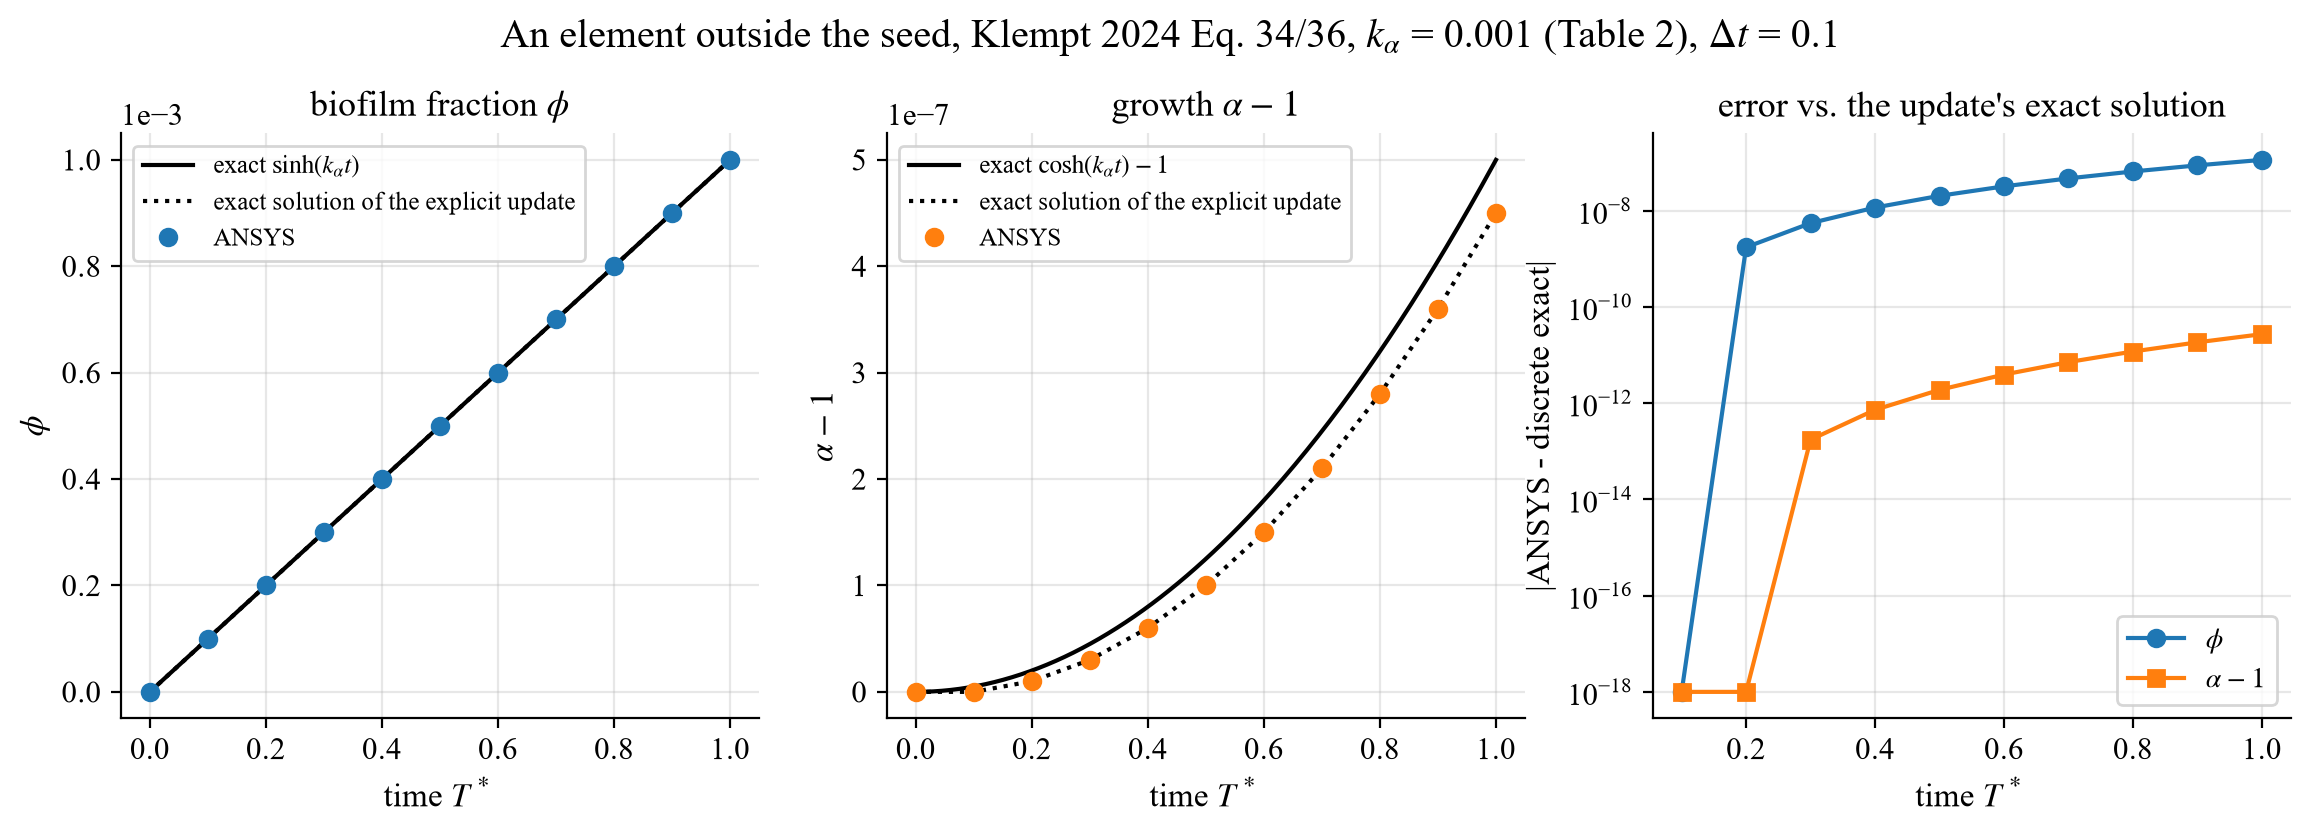
\includegraphics[width=0.95\linewidth,height=0.64\textheight,keepaspectratio]{fig1005_exact.png}
\takeaway{Where $\phi$ has no gradient, $\phi=\sinh(k_\alpha t)$ and $\alpha-1=\cosh(k_\alpha t)-1$:
ANSYS follows the exact solution of the time stepping to $3\times10^{-11}$ in $\alpha$.}
\end{frame}

% --------------------------------------------------------
\begin{frame}{Part 2: stresses with the published stiffness}
\begin{columns}[T]
\begin{column}{0.56\textwidth}
\centering
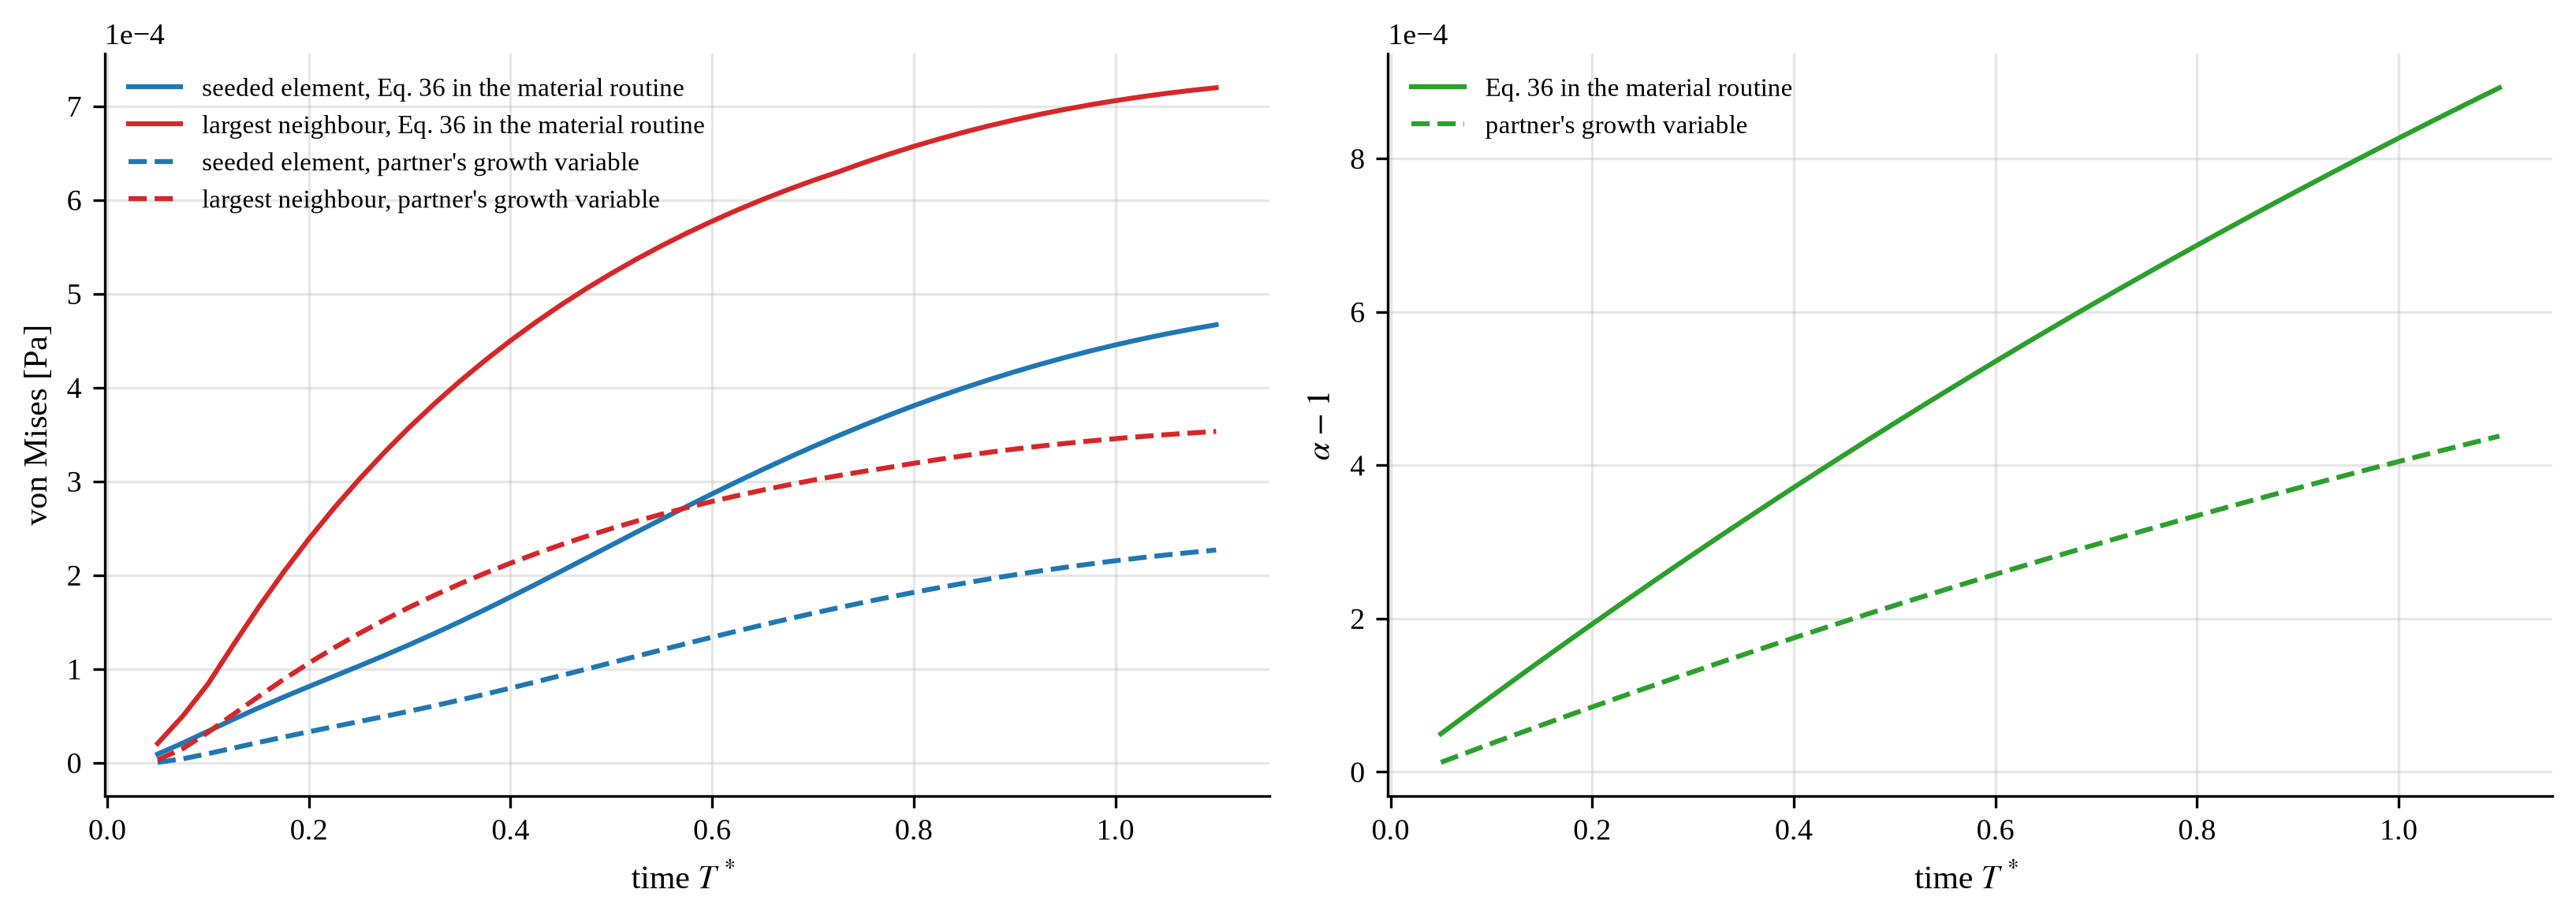
\includegraphics[width=\linewidth,height=0.7\textheight,keepaspectratio]{fig_element_beta002.png}
\end{column}
\begin{column}{0.42\textwidth}
\small
At $T^*=1.1$ on $16^3$ elements:\\[3pt]
\begin{tabular}{@{}lr@{}}
\toprule
mean stress, seed & $-2.5\times10^{-4}$~Pa\\
mean stress, first layer & $+6.0\times10^{-5}$~Pa\\
von Mises, seed mean & $5.9\times10^{-4}$~Pa\\
$\alpha-1$ in the seed & $8.9\times10^{-4}$\\
\bottomrule
\end{tabular}\\[6pt]
Stresses scale with $E=10$~Pa.
\end{column}
\end{columns}
\takeaway{The seed is compressed and the material around it is in tension: the ring of tension of Klempt et al.\ 2024.}
\end{frame}

% --------------------------------------------------------
\begin{frame}{Part 2: how far the numbers can be trusted}
\begin{columns}[T]
\begin{column}{0.58\textwidth}
\centering
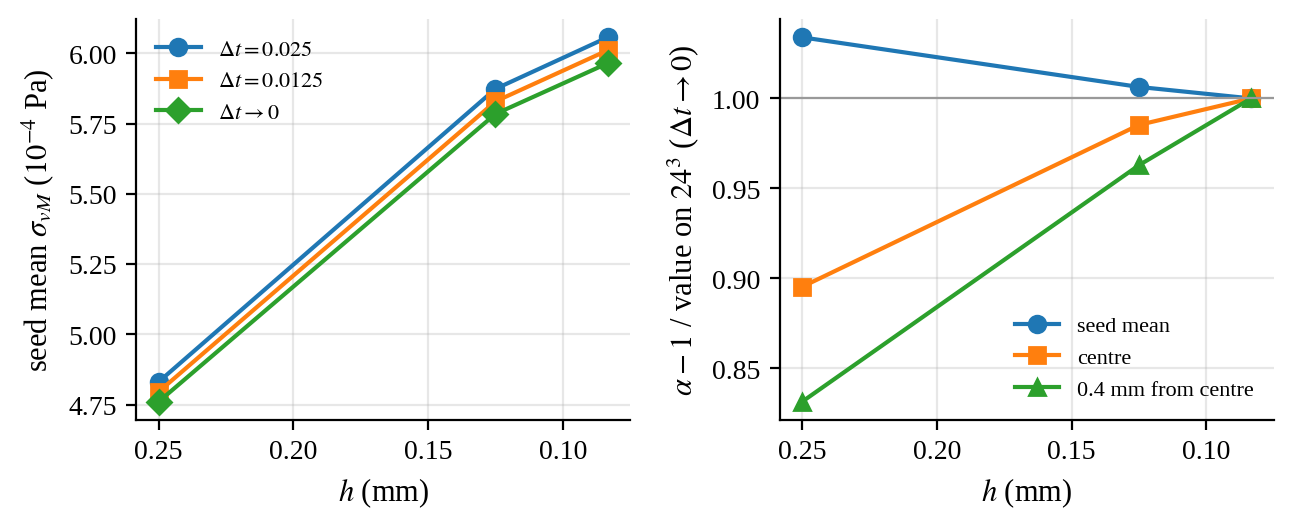
\includegraphics[width=\linewidth,height=0.72\textheight,keepaspectratio]{fig_wp3_convergence.png}
\end{column}
\begin{column}{0.4\textwidth}
\small
\begin{itemize}
  \item Time: first order; $\Delta t=0.025$ gives about $1\,\%$
  \item Mesh: seed stress converges at an observed order of about $2$;
        error on $24^3$ about $2\,\%$ (three meshes only)
  \item $\alpha-1$ at fixed positions: $16^3\to24^3$ within $4\,\%$
  \item Explicit field update: smooth up to $\beta\Delta t/h^2=0.144$,
        oscillating at $0.160$; stricter than $h^2/(2\Delta t)\ge\beta$
        (Rudolf et al.\ 2025)
\end{itemize}
\end{column}
\end{columns}
\takeaway{Seed stresses on $24^3$ elements are good to about $2\,\%$; every run of the thesis is inside the stability limit.}
\end{frame}

% --------------------------------------------------------
\begin{frame}{Part 3: composition at every Gauss point}
\begin{columns}[T]
\begin{column}{0.5\textwidth}
\small
\begin{itemize}
  \item Two species, cases of Klempt et al.\ 2026
  \item Every call from ANSYS to the point model is reproduced in Python
        bit for bit
  \item Packed seed, $\phi_1/(\phi_1+\phi_2)$ at $T^*=1$:
        case~3 (coexistence) $0.667$, case~6 (one species wins) $0.021$;
        the type of outcome is kept
  \item \textcolor{warn}{Assumptions} (not in the papers), each with its
        sensitivity: time link $s=0.15$, cap $\phi_{\rm cap}=0.9$,
        threshold $\phi_{\min}=0.01$
\end{itemize}
\end{column}
\begin{column}{0.48\textwidth}
\centering
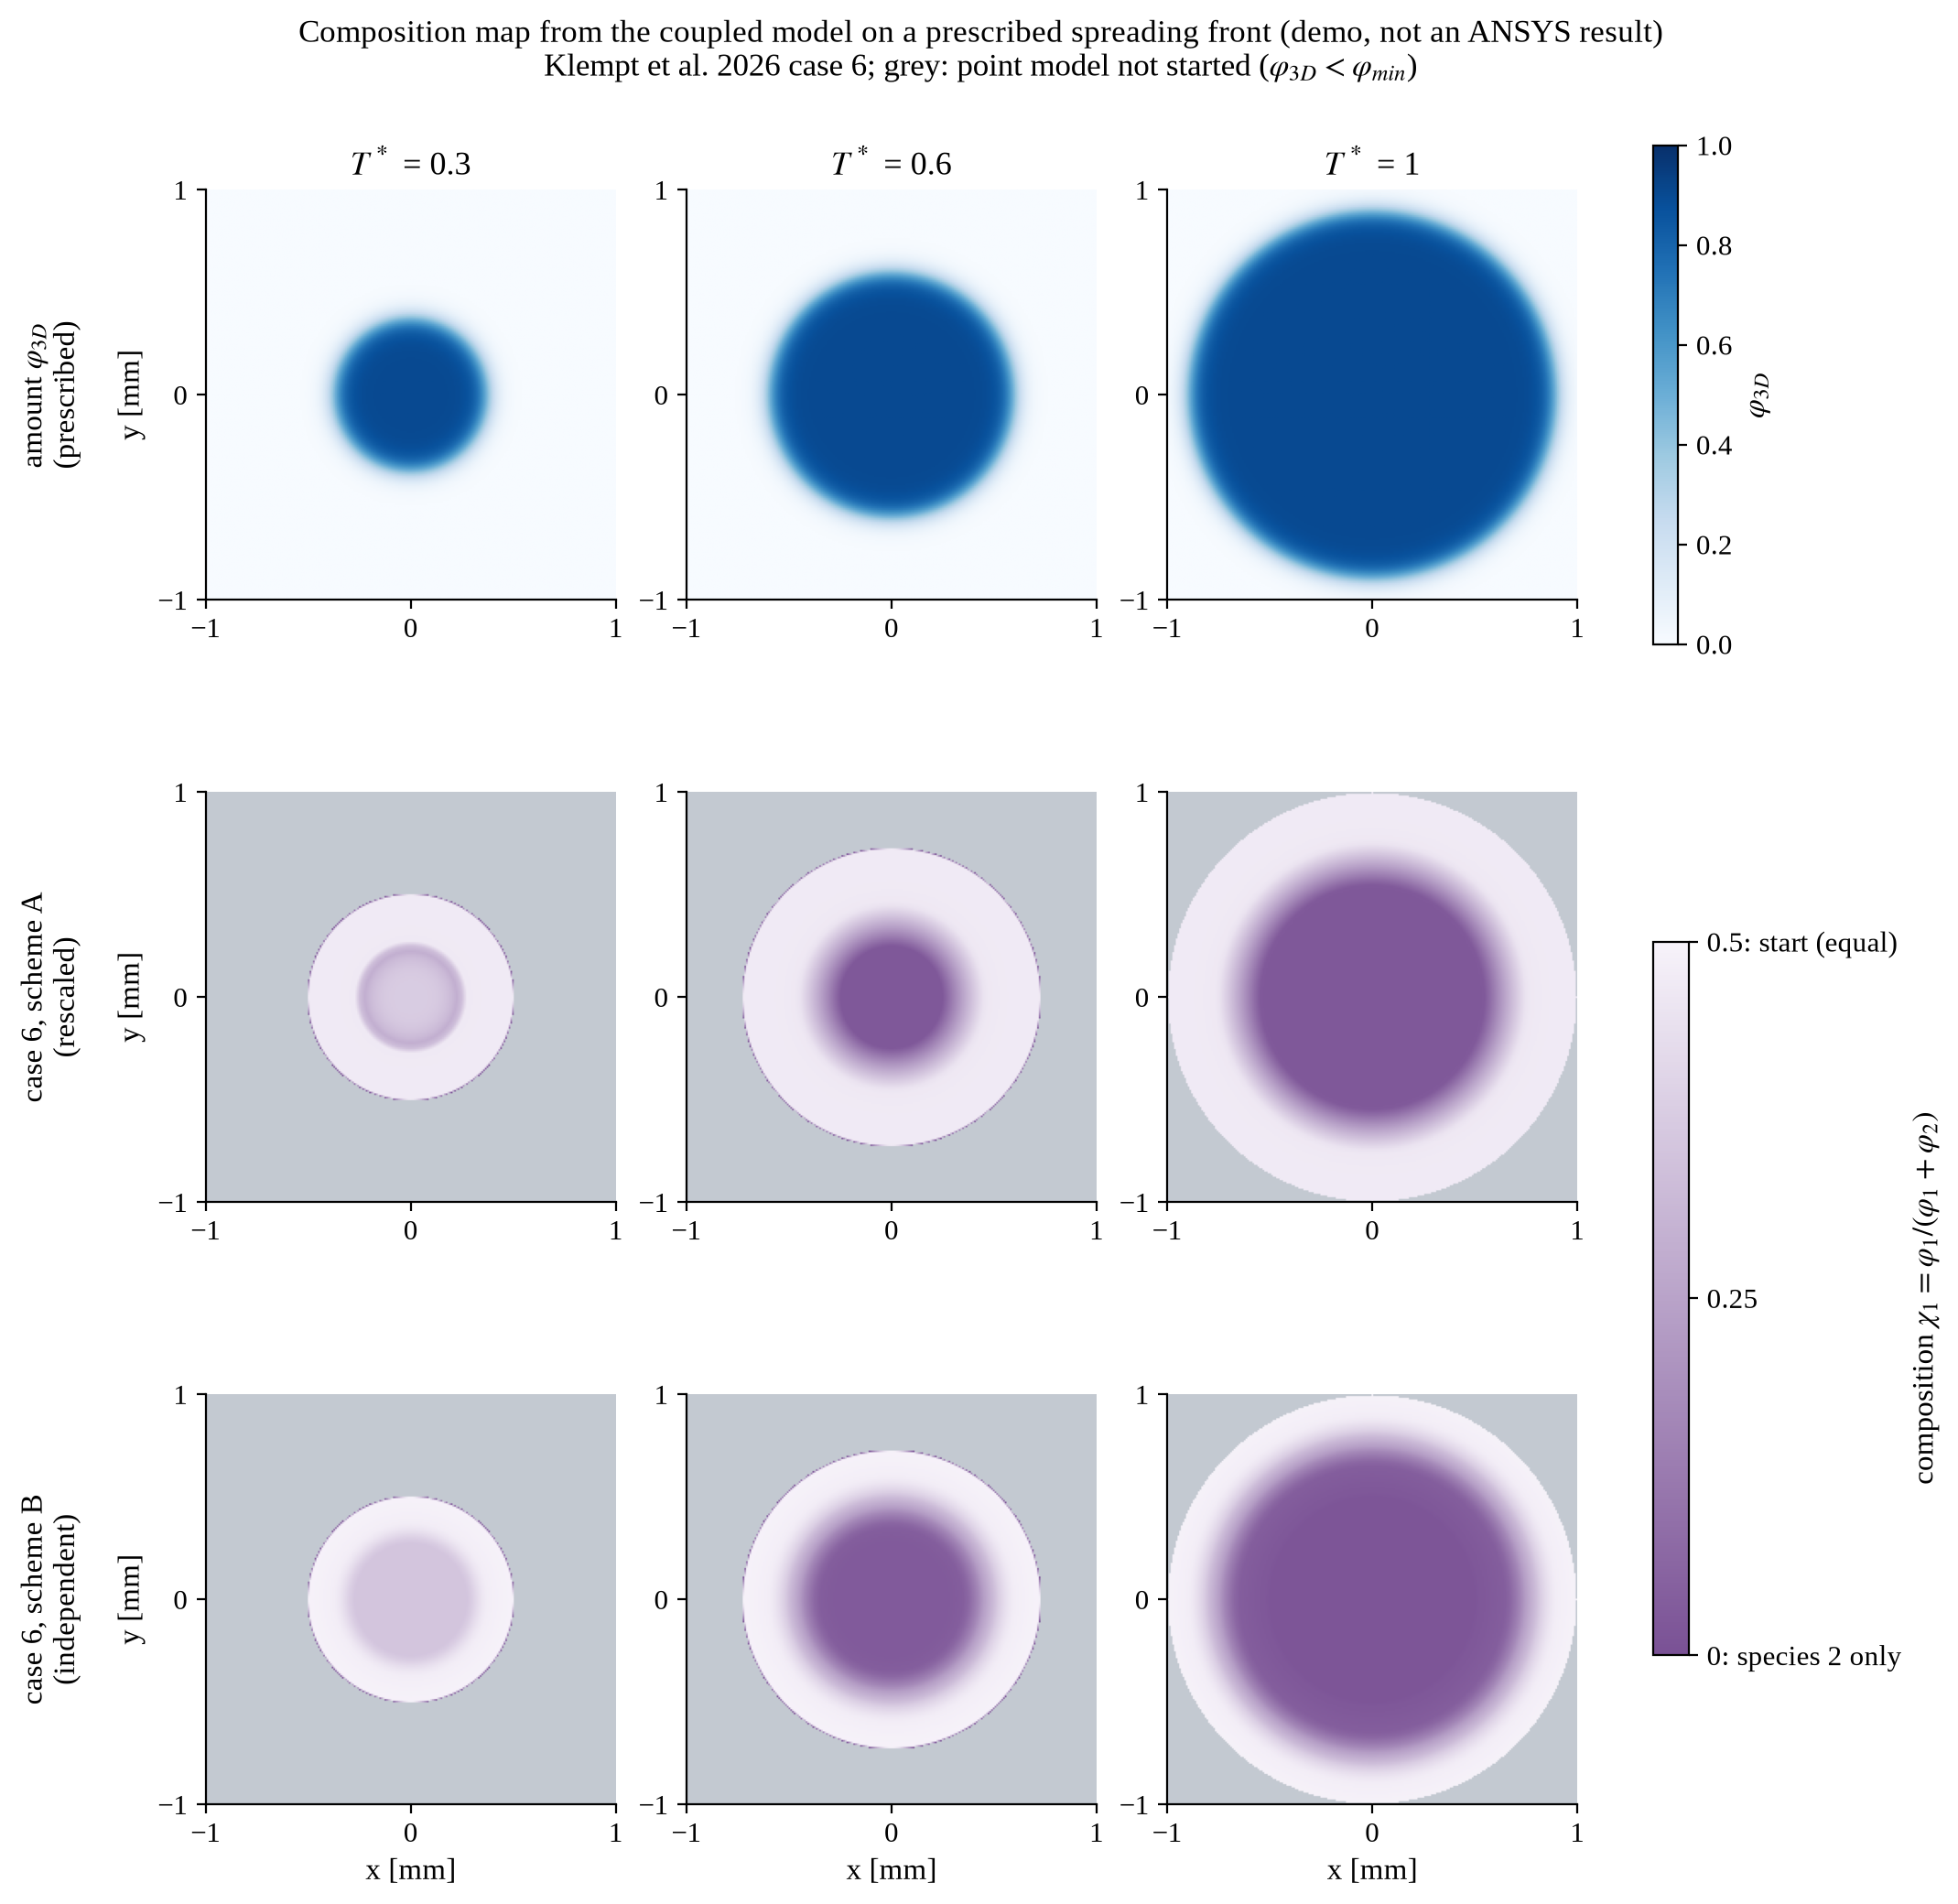
\includegraphics[width=\linewidth,height=0.66\textheight,keepaspectratio]{fig_composition_map.png}
\end{column}
\end{columns}
\takeaway{The coupled run keeps the published outcomes: coexistence in case~3, one surviving species in case~6.}
\end{frame}

% --------------------------------------------------------
\begin{frame}{Part 3: composition varies in space with the local nutrient}
\centering
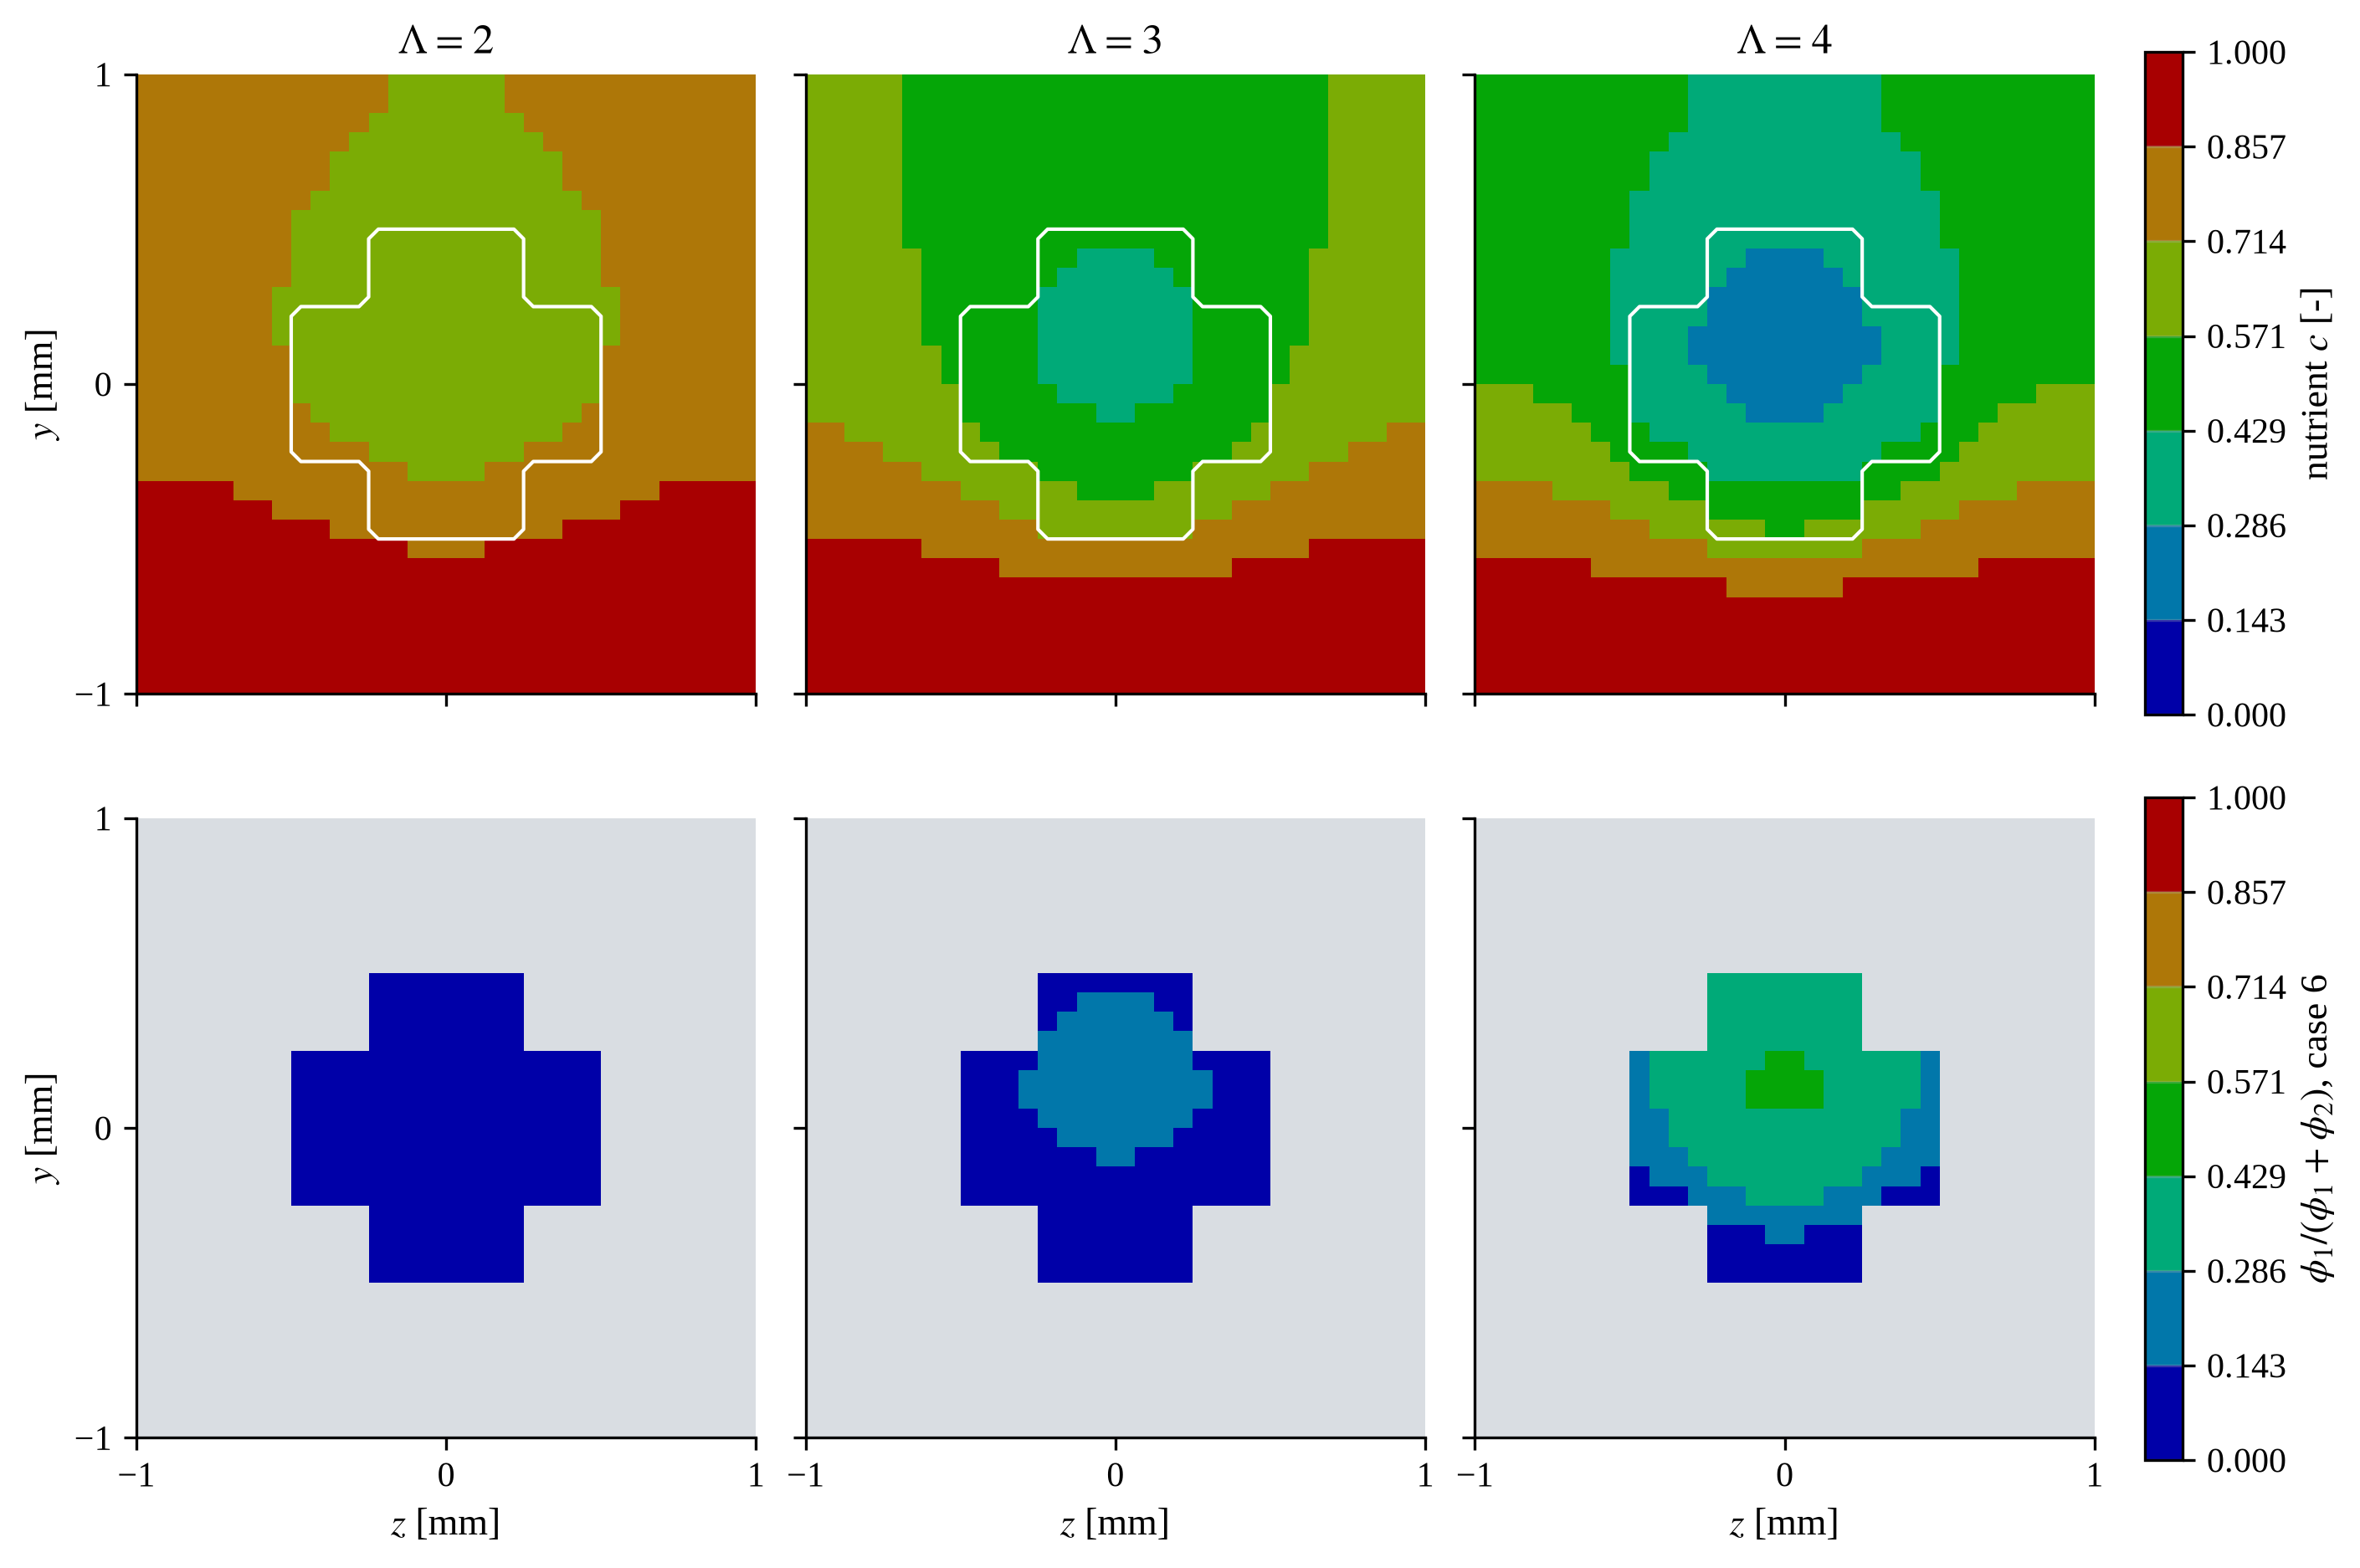
\includegraphics[width=\linewidth,height=0.6\textheight,keepaspectratio]{fig_composition_local_nutrient_thesis.png}\\
\small Nutrient held at one face, consumed in the seed; Thiele number
$\Lambda^2=gL^2/d$. Case~6 at $\Lambda=4$: share $0.03$ near the nutrient,
$0.44$ inside; case~3 hardly changes ($0.63$--$0.66$).
\takeaway{With a local nutrient the composition varies in space, which a constant $c^*$ cannot show.}
\end{frame}

% --------------------------------------------------------
\begin{frame}{Limitations}
\begin{itemize}
  \item \textbf{Verification, not validation}: no measured stress of a growing
        oral biofilm was available
  \item \textbf{One-way}: the composition does not act on stiffness, spreading
        or stress (as in Klempt et al.\ 2024)
  \item \textbf{No spreading towards the nutrient in ANSYS}: the front term of
        the element is inactive
  \item \textbf{Assumptions}: the time link $s$, $\phi_{\rm cap}$, the
        conversion of $\beta$; each reported with its sensitivity
  \item \textbf{Calibration and element not yet joined}: five calibrated species
        in Part~1, two published cases in Part~3
  \item \textbf{Symmetric $\mathbf A$}: no directed effects; different
        \textit{P.~gingivalis} strains in the commensal and dysbiotic data
\end{itemize}
\end{frame}

% --------------------------------------------------------
\begin{frame}{Conclusion and outlook}
\begin{columns}[T]
\begin{column}{0.5\textwidth}
\textbf{Done}\\[3pt]
\small
\cbox{p1}{1.15cm}{\textbf{\color{p1}1 Calibration:} five species, four conditions; pH predicted out of sample ($R^2=0.78$)}\\[3pt]
\cbox{p2}{1.15cm}{\textbf{\color{p2}2 Growth law:} Klempt et al.\ 2024 in the IKM element, verified to $3\times10^{-11}$}\\[3pt]
\cbox{p3}{1.15cm}{\textbf{\color{p3}3 Composition:} two species at every Gauss point, published outcomes kept}
\end{column}
\begin{column}{0.48\textwidth}
\textbf{Next (Keio University)}
\begin{itemize}\small
  \item Five calibrated species in the element
  \item Composition into stiffness, stress into growth (two-way)
  \item A working front term; explicit against implicit field update
  \item Posterior uncertainty carried to the stress
\end{itemize}
\end{column}
\end{columns}
\vspace{10pt}
\centering\large Thank you.
\end{frame}

% --------------------------------------------------------
\begin{frame}{References}
\footnotesize
\begin{itemize}
  \item F.~Klempt, M.~Soleimani, P.~Wriggers, P.~Junker (2024), Biomech.\
        Model.\ Mechanobiol.\ 23, 2091--2113: growth field, Eq.~34/36, Table~2
  \item F.~Klempt, H.~Geisler, M.~Soleimani, P.~Junker (2026), Arch.\ Appl.\
        Mech.\ 96, 164: multi-species point model
  \item P.~Junker, D.~Balzani (2021), Contin.\ Mech.\ Thermodyn.\ 33,
        1931--1956: extended Hamilton principle
  \item P.~Junker, J.~Makowski, K.~Hackl (2014), Contin.\ Mech.\ Thermodyn.\
        26, 259--268; K.~Hackl (1997), J.\ Mech.\ Phys.\ Solids 45, 667--688
  \item T.~Rudolf et al.\ (2025), Finite Elem.\ Anal.\ Des.\ 249, 104353:
        Neighbored Element Method
  \item N.~Heine et al.\ (2025), Front.\ Oral Health: in-vitro data
  \item D.~Feng et al.\ (2021), Bull.\ Math.\ Biol.\ 83, 48;
        M.~Soleimani et al.\ (2023), Sci.\ Rep.: two-species models
\end{itemize}
\end{frame}

\appendix
% --------------------------------------------------------
\begin{frame}{Appendix A: notation}
\scriptsize
\begin{columns}[T]
\begin{column}{0.5\textwidth}
\textbf{Growth field and mechanics (Klempt et al.\ 2024)}\\[2pt]
\begin{tabular}{@{}ll@{}}
\toprule
$\phi$, $\phi_{3D}$ & amount of biofilm (0 = void, 1 = dense)\\
$c$ & nutrient concentration\\
$\alpha$ & $\mathbf F_g=\alpha\mathbf I$, $\alpha(0)=1$; growth is $\alpha-1$\\
$\mathbf F=\mathbf F_e\mathbf F_g$ & elastic / growth split\\
$k_\alpha$ & growth rate ($10^{-3}\,T^{*-1}$)\\
$\beta$ & diffusion of $\phi$ ($0.02$~mm$^2/T^*$, converted)\\
$d$, $g$ & nutrient diffusivity, consumption\\
$r$, $k$ & front growth parameter, half-velocity constant\\
$E$, $\nu$ & $10$~Pa, $0.49$ (Klempt 2024, Table~2)\\
$T^*$ & normalised time\\
\bottomrule
\end{tabular}
\end{column}
\begin{column}{0.48\textwidth}
\textbf{Point model (Klempt et al.\ 2026)}\\[2pt]
\begin{tabular}{@{}ll@{}}
\toprule
$\phi_i$, $\phi_0$ & volume fraction of species $i$, void\\
$\psi_i$, $\bar\phi_i$ & viability, living fraction $\phi_i\psi_i$\\
$A_{ij}$ & symmetric interaction matrix\\
$c^*$, $\alpha^*$ & nutrient, antibiotic level\\
$\eta_i$ & dissipation parameters\\
$\gamma$ & multiplier of $\sum_l\phi_l=1$\\
\bottomrule
\end{tabular}\\[6pt]
\textbf{Coupling (this work)}\\[2pt]
\begin{tabular}{@{}ll@{}}
\toprule
$\phi_1/(\phi_1+\phi_2)$ & composition (share of species 1)\\
$s$ & point model advances $s\,\Delta t$ per substep\\
$\phi_{\rm cap}$, $\phi_{\min}$ & cap on the amount, start threshold\\
$\lambda=\beta\Delta t/h^2$ & stability measure\\
\bottomrule
\end{tabular}
\end{column}
\end{columns}
\end{frame}

% --------------------------------------------------------
\begin{frame}{Appendix B: growth field and mechanics}
\small
\textbf{Kinematics.} $\mathbf F=\mathbf F_e\mathbf F_g$ with isotropic
$\mathbf F_g=\alpha\mathbf I$. Stress comes only from $\mathbf F_e$. A body
that can grow freely stays stress free; stress appears where growth is
constrained.\\[3pt]
\textbf{Material.} $E(\phi)=(\phi^2+f)\,E$, $E=10$~Pa, $\nu=0.49$
(Klempt 2024, Table~2; their material is incompressible), $f=10^{-3}$;
decks in mm and MPa, stresses quoted in Pa.\\[3pt]
\textbf{Field equations} (Klempt et al.\ 2024, Eqs.~34--36, without the bars):
\[
\dot\phi=\underbrace{\beta\,\nabla^2\phi}_{\text{diffusion}}
+\underbrace{k_\alpha\,\alpha}_{\text{local source}}
-\underbrace{\|\nabla\phi\|\,\frac{r\,c}{k+c}\,\mathbf n_{\nabla\phi}\cdot\mathbf n_{\nabla c}}_{\text{front, inactive in ANSYS}},
\qquad
\dot c=d\,\nabla^2c-g\,\phi\,c,
\qquad
\dot\alpha=k_\alpha\,\phi
\]
\begin{itemize}
  \item $\phi$ and $c$ are fields of the element, updated explicitly with the
        Neighbored Element Method; $\alpha$ is a state variable at the Gauss points
  \item Consumption $g\phi c$ as in the authors' implementation (printed:
        $g\phi$)
\end{itemize}
\end{frame}

% --------------------------------------------------------
\begin{frame}{Appendix C: point model and one coupled substep}
\small
\textbf{Point model} (Klempt et al.\ 2026), per species $i$, no space:
\[
\begin{aligned}
(\eta_{\phi,i}+\eta_i\psi_i^2)\,\dot\phi_i+\eta_i\phi_i\psi_i\,\dot\psi_i
&= c^*\psi_i\textstyle\sum_j A_{ij}\phi_j\psi_j-\gamma-(\text{barrier})\\
\eta_i\,(\phi_i\psi_i\,\dot\phi_i+\phi_i^2\,\dot\psi_i)
&= c^*\phi_i\textstyle\sum_j A_{ij}\phi_j\psi_j-\alpha^* b_i\,\psi_i-(\text{barrier})
\end{aligned}
\]
with $\sum_i\phi_i+\phi_0=1$; the barrier keeps $\phi_i,\psi_i$ in $(0,1)$;
implicit Euler and Newton, $\Delta t=10^{-4}$.\\[4pt]
\textbf{One substep of the coupled ANSYS run}
\begin{enumerate}
  \item The element updates its field $\phi$
  \item At each Gauss point: $\alpha_{n+1}=\alpha_n+k_\alpha\phi\,\Delta t$,
        $\mathbf F_g=\alpha\mathbf I$, stress and tangent
  \item Two species, where $\phi_{3D}\ge\phi_{\min}$: scale the point model to
        $\min(\phi_{3D},\phi_{\rm cap})$, advance it by $s\,\Delta t$, store
        $\phi_i,\psi_i$ as state variables
\end{enumerate}
\end{frame}

% --------------------------------------------------------
\begin{frame}{Appendix D: stability of the explicit field update}
\centering
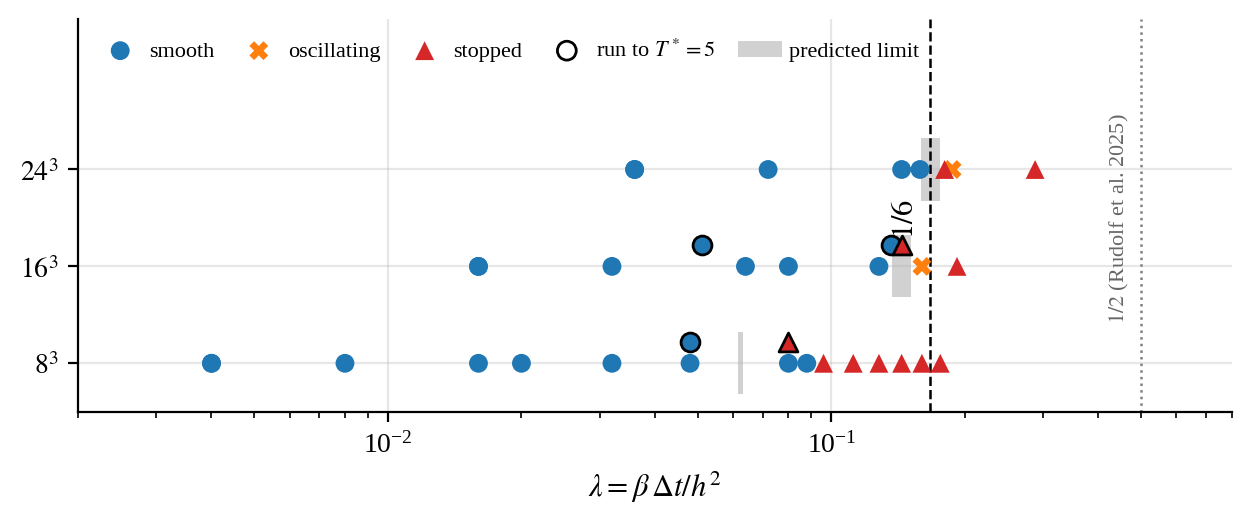
\includegraphics[width=0.95\linewidth,height=0.55\textheight,keepaspectratio]{fig_wp3_stability.png}\\
\small $\lambda=\beta\Delta t/h^2$. Smooth up to $0.144$, oscillating at $0.160$, elements
collapse above. Dashed: $1/6$ of the seven-point stencil; dotted: $1/2$ from
$h^2/(2\Delta t)\ge\beta$ (Rudolf et al.\ 2025). All runs of the thesis: $\lambda\le0.128$.
\end{frame}

\end{document}
